\documentclass{article}
\usepackage{graphicx}
\usepackage[sharp]{easylist}
\usepackage[utf8]{inputenc}
\usepackage[left=3.5cm, right=3.5cm]{geometry}

\graphicspath{ {images/} }
\title{A short description of the Chess Application}
\author{Group 6}
\date{19-02-2018}

\begin{document}
\maketitle

\section*{The Chess Application}

This chess game focuses on giving players of any age the chance to play classic chess digitally. The application has easy to use controls and comes with all functionality of a regular chessboard, with the choice of challenging a computer controlled opponent or another human.

\section*{System Requirements}
\paragraph{Supported Platforms}\mbox{}\\
\begin{easylist}[itemize]
    # Windows 10 or above
    # Mac OSX High Sierro or above
    # Ubuntu Linux
\end{easylist}
\paragraph{Hardware requirements}\mbox{}\\
\begin{easylist}[itemize]
    # Processor : 32-bit or greater
    # More than 512 MB RAM
\end{easylist}
\paragraph{Software requirements}\mbox{}\\
\begin{easylist}[itemize]
    # Java SE 8 or greater
\end{easylist}

\newpage

\section*{How to play}
\subsection*{Basics}

The board consists of 8x8 squares, with the starting position as shown in figure 1. White always goes first.

\noindent There are 6 types of pieces: \\
\begin{easylist}[itemize]
    # The king can only move 1 step in any direction. If it is taken, the owner has lost the game. See figure 2.
    # The rooks can move any length horizontally and vertically. See figure 3.
    # Bishops can move any length diagonally. See figure 4.
    # The queen can move any length in any direction. See figure 5.
    # Knights can move either 2 squares horizontally and then one square vertically, or 2 squares vertically and then one square horizontally. See figure 6.
    # Pawns can move one step forwards, or two steps forward if in the starting position. Unlike the other pieces it can only hit a piece one step up vertically to left or right. See figure 7.
\end{easylist}

\begin{figure}[!htb]
\minipage{0.32\textwidth}%
  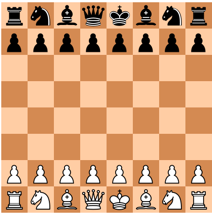
\includegraphics[width=\linewidth]{chess1}
  \caption{Starting position}\label{fig:chess1}
\endminipage\hfill
\minipage{0.32\textwidth}%
  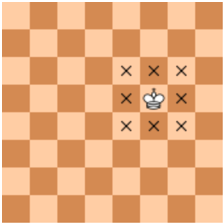
\includegraphics[width=\linewidth]{chess2}
  \caption{King}\label{fig:chess2}
\endminipage\hfill
\minipage{0.32\textwidth}%
  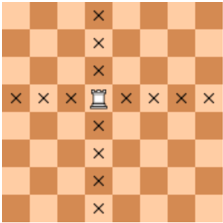
\includegraphics[width=\linewidth]{chess3}
  \caption{Rook}\label{fig:chess3}
\endminipage
\end{figure}
\begin{figure}[!htb]
\minipage{0.32\textwidth}%
  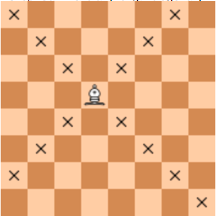
\includegraphics[width=\linewidth]{chess4}
  \caption{Bishop}\label{fig:chess4}
\endminipage\hfill
\minipage{0.32\textwidth}%
  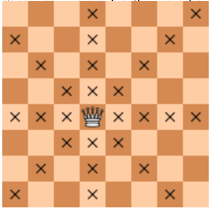
\includegraphics[width=\linewidth]{chess5}
  \caption{Queen}\label{fig:chess5}
\endminipage\hfill
\minipage{0.32\textwidth}%
  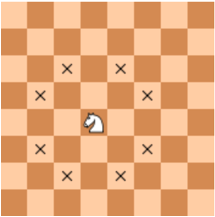
\includegraphics[width=\linewidth]{chess6}
  \caption{Knight}\label{fig:chess6}
\endminipage
\end{figure}

\newpage
\subsection*{Special moves}
\textbf{Castling:} The king moves two steps either to the right or to the left. The Rook then “jumps over” the king and is placed in the field adjacent to the King. For this move to be possible all the fields between the King and the Rook needs to be empty. The King and Rook must be in the starting position, never having moved. The Rook, King and the fields between them cannot be under “attack” such that another piece would be able to hit the piece if it was the opponents turn. See figure 7 and 8. \\

\noindent\textbf{En passant:} If the opponents pawn moves two steps forward from the starting position, and is thus 
Placed next to your won pawn, you are strike it as if it had only moved one step forward. See figure 9 and 10.


\begin{figure}[!htb]
\minipage{0.32\textwidth}%
    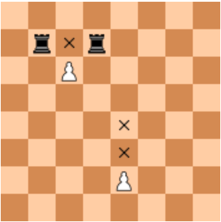
\includegraphics[width=\linewidth]{chess7}
    \caption{Before castling}\label{fig:chess7}
\endminipage\hfill
\minipage{0.32\textwidth}%
    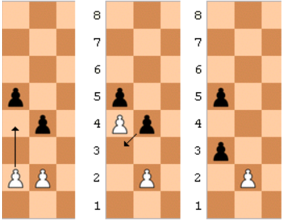
\includegraphics[width=\linewidth]{chess10}
    \caption{After castling}\label{fig:chess8}
\endminipage
\end{figure}
\begin{figure}[!htb]
\minipage{0.32\textwidth}%
    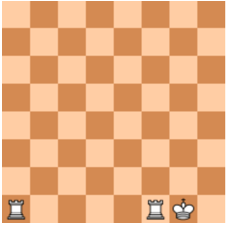
\includegraphics[width=\linewidth]{chess8}
    \caption{En passant 1}\label{fig:chess9}
\endminipage\hfill
\minipage{0.32\textwidth}%
    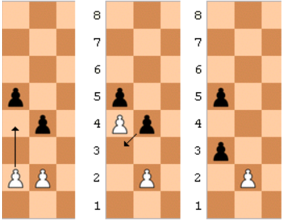
\includegraphics[width=\linewidth]{chess10}
    \caption{En passant 2}\label{fig:chess10}
\endminipage
\end{figure}

\end{document}